\documentclass{article}


% if you need to pass options to natbib, use, e.g.:
% \PassOptionsToPackage{numbers, compress}{natbib}
% before loading nips_2016
%
% to avoid loading the natbib package, add option nonatbib:
% \usepackage[nonatbib]{nips_2016}

%\usepackage{nips_2016}

% to compile a camera-ready version, add the [final] option, e.g.:
\usepackage[final]{nips_2016}

\usepackage[utf8]{inputenc} % allow utf-8 input
\usepackage[T1]{fontenc}    % use 8-bit T1 fonts
\usepackage{hyperref}       % hyperlinks
\usepackage{url}            % simple URL typesetting
\usepackage{booktabs}       % professional-quality tables
\usepackage{amsfonts}       % blackboard math symbols
\usepackage{nicefrac}       % compact symbols for 1/2, etc.
\usepackage{microtype}      % microtypography
\usepackage{graphicx}
\usepackage{wrapfig}
%\usepackage{caption}
\usepackage{subcaption}
\usepackage{bm}

\def\code#1{\texttt{#1}}

\title{Solution for Project \#2 \\\large Deep Learning, HHU 2016 / 2017 }




% The \author macro works with any number of authors. There are two
% commands used to separate the names and addresses of multiple
% authors: \And and \AND.
%
% Using \And between authors leaves it to LaTeX to determine where to
% break the lines. Using \AND forces a line break at that point. So,
% if LaTeX puts 3 of 4 authors names on the first line, and the last
% on the second line, try using \AND instead of \And before the third
% author name.

\author{
  Thomas Germer \\
  \And
  Michael Janschek \\
  \And
  Patrick Brzoska \\
    %% Affiliation \\
  %% Address \\
  %% \texttt{email} \\
  %% \AND
  %% Coauthor \\
  %% Affiliation \\
  %% Address \\
  %% \texttt{email} \\
  %% \And
  %% Coauthor \\
  %% Affiliation \\
  %% Address \\
  %% \texttt{email} \\
  %% \And
  %% Coauthor \\
  %% Affiliation \\
  %% Address \\
  %% \texttt{email} \\
}

\begin{document}
\maketitle

\section{Code and Architecture}

The code is provided as GitHub repository and is available under
\begin{center}
	\url{https://github.com/99991/DeepLearningProjects/tree/master/projects/project2}
\end{center}

%To test various neural network configurations, run
%\begin{center}
%	\url{https://github.com/99991/DeepLearningProjects/blob/master/projects/test/test_runner.py}
%\end{center}

\newpage

\section{Tasks}

\begin{enumerate}
	\begin{item}
		\textbf{CNN on CIFAR-10}
	\end{item}

	\begin{enumerate}
		
		
		%a)
		\begin{item}
			To accommodate the higher complexity of the CIFAR-10 dataset we chose to train a relatively deep CNN compared to our first project.  
			Also, with the number of batches at 10000 and each batch having 64 samples, the training time was increased.
			
			The leaky Rectified Linear Unit (ReLU) activation function was used to counter the "dying ReLU" problem. Instead of the function being zero when $x < 0$, it is set to a small negative value of $ 0.1 * x $. 
		\end{item}
		
		
		%b)
		\begin{item}
		\begin{figure}
		\centering
			\begin{subfigure}[b]{0.45\textwidth}
				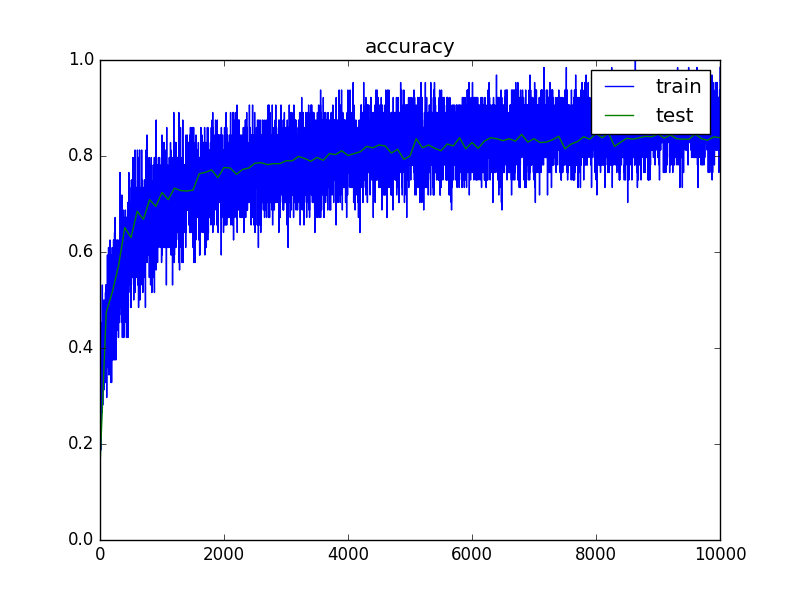
\includegraphics[width=\textwidth]{figures/accuracy_32kernels}
				\caption{accuracy}
				\label{fig:basic_accu}
			\end{subfigure}	
			\quad
			\begin{subtable}[b]{0.4\textwidth}
				\begin{tabular}{lll}
        					\toprule
        					Parameter     & Value \\
        					\midrule
        					batch\_size & 64  \\
        					num\_batches & 10001  \\
        					kernel\_size &3 \\
        					num\_kernels & 32 \\
        					num\_hidden & 500 \\
        					depth & 3 \\
        					dropout\_keep\_probability & 0.5 \\
        					\bottomrule
     				\end{tabular}
				\caption{Basic configuration}
				\label{basic_config}
			\end{subtable}
			\caption{Performance and parameters for our basic configuration}
		\end{figure}
		
		Table \ref{basic_config} shows the configuration of our network, while figure \ref{fig:basic_accu} shows its achieved accuracy.		
			With these parameters a test accuracy of 82.8\% was reached, which seems to be a fairly good number compared to other implementations.
			
		\end{item}
		
		
		
		%c)
		\begin{item}
		\begin{figure}
		\centering
			\begin{subfigure}[b]{0.45\textwidth}
				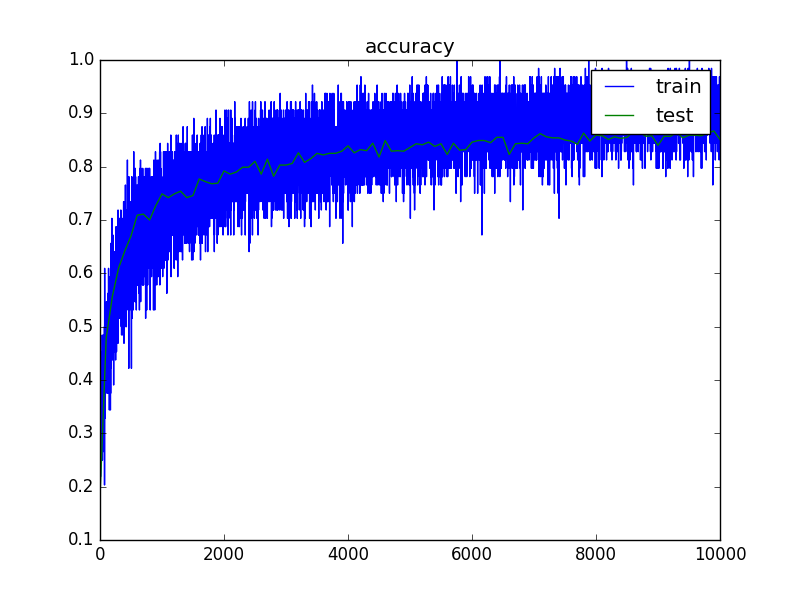
\includegraphics[width=\textwidth]{figures/accuracy_64kernels}
				\caption{64 kernels}
				\label{fig:64kern}
			\end{subfigure}	
			\quad
			\begin{subfigure}[b]{0.45\textwidth}
				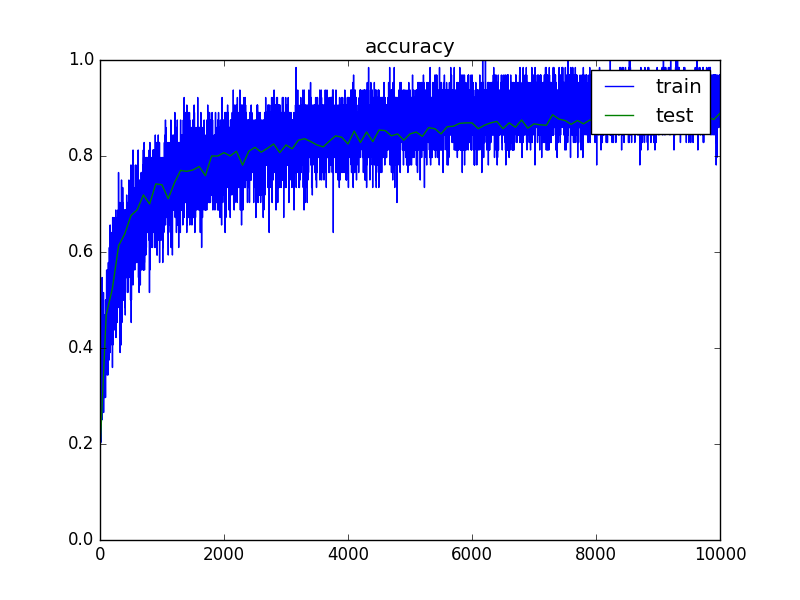
\includegraphics[width=\textwidth]{figures/accuracy_128kernels}
				\caption{128 kernels}
				\label{fig:128kern}
			\end{subfigure}	
			\quad
			\begin{subtable}[b]{0.4\textwidth}
				\begin{tabular}{lll}
        					\toprule
        					number of batches & number of kernels    & Accuracy \\
        					\midrule
        					30000  & 32 & 87\%  \\
        					10000  & 64 & 85.1\%  \\
					10000 &128 & 88.9\%  \\
					14200  & 128 & 91.6\%  \\
					\bottomrule
     				\end{tabular}
				\caption{Increase of iterations and kernels}
				\label{kernels}
			\end{subtable}
			\caption{Accuracy for various parameter configurations}
		\end{figure}
		
			By increasing the number of batches to 30000 a test accuracy of 87\% was achieved. Increasing the kernel size to 64 while retaining a batch size of 10000 was not as successful, but still reached an accuracy of 85.1\%. A kernel size of 128 resulted in an even higher test accuracy of 88.9\%. The network even reached a test accuracy of  91.6\% when increasing the batch size to 14200 with 128 kernels.
		\end{item}
		
		
		
		
		%d)
		\begin{item}
			In 
			\citet{Zagoruyko:2016aa} 
			average pooling has yielded better results, but max pooling has worked better within our network.
			Also, using global average pooling as a regularizer as in 
			\citet{Lin:2013aa} 
			has not had a positiv effect on the test accuracy.
			
		\end{item}
		
		
		
		%e)
		\begin{item}
			Using random cropping as a way to increase the data size has lead to minor improvements. 
			Random brightness and saturation has not yielded any success.
		\end{item}
		
		
		
		%f)
		\begin{item}
			Adding dropout has not resulted in any success. With the configuration shown in  \ref{basic_config} adding dropout resulted in a test accuracy of 74.8\%.
		\end{item}
		
		
		
		%g)
		\begin{item}
			Please see  figure \ref{fig:tensorboard}. 

		\end{item}
		
		
	\end{enumerate}


%%%%%%%%%%%%%%%%%%%%%


		\begin{figure}[t]
			\centering
			\begin{subfigure}[b]{0.45\textwidth}
				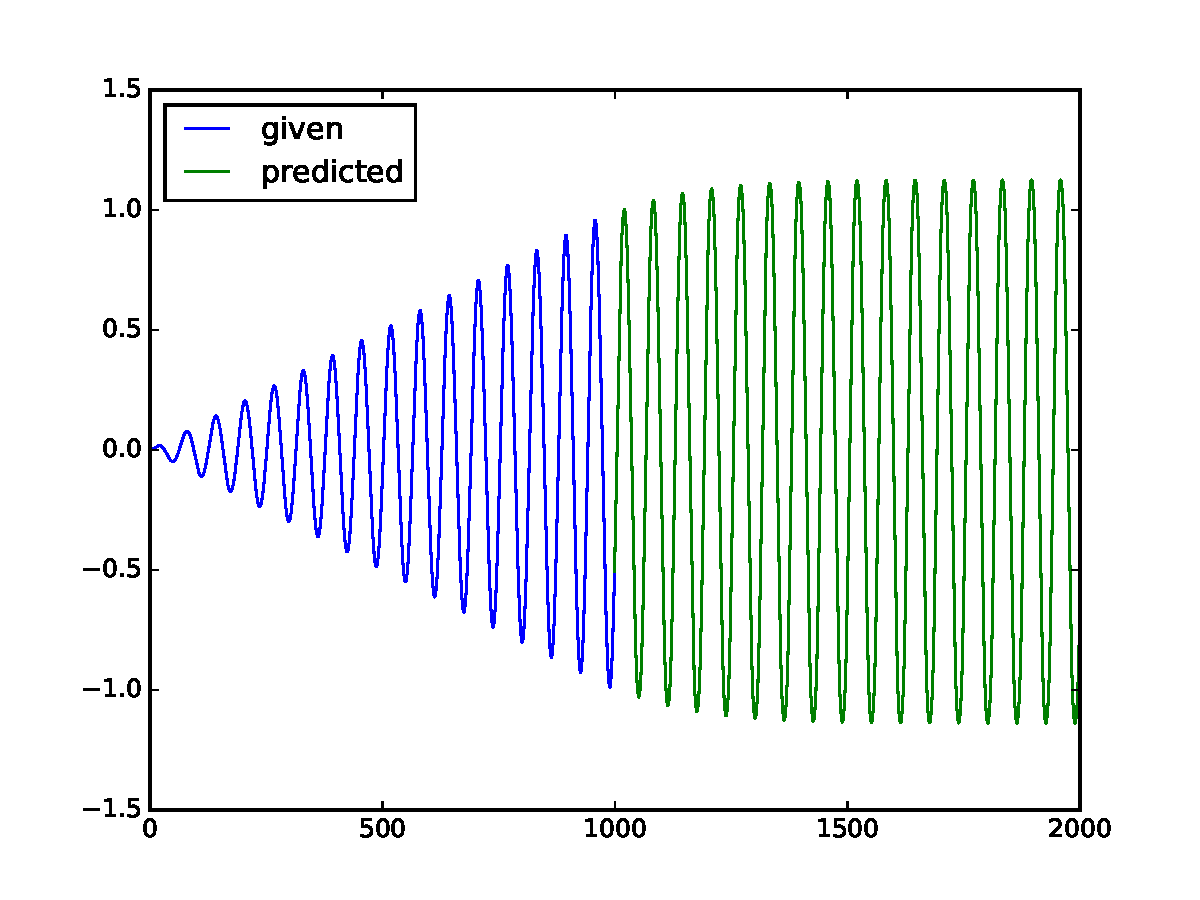
\includegraphics[width=1\textwidth]{figures/sine}
				\caption{Sine wave}
				\label{fig:sine}
			\end{subfigure}	
			\quad
			\begin{subfigure}[b]{0.45\textwidth}
				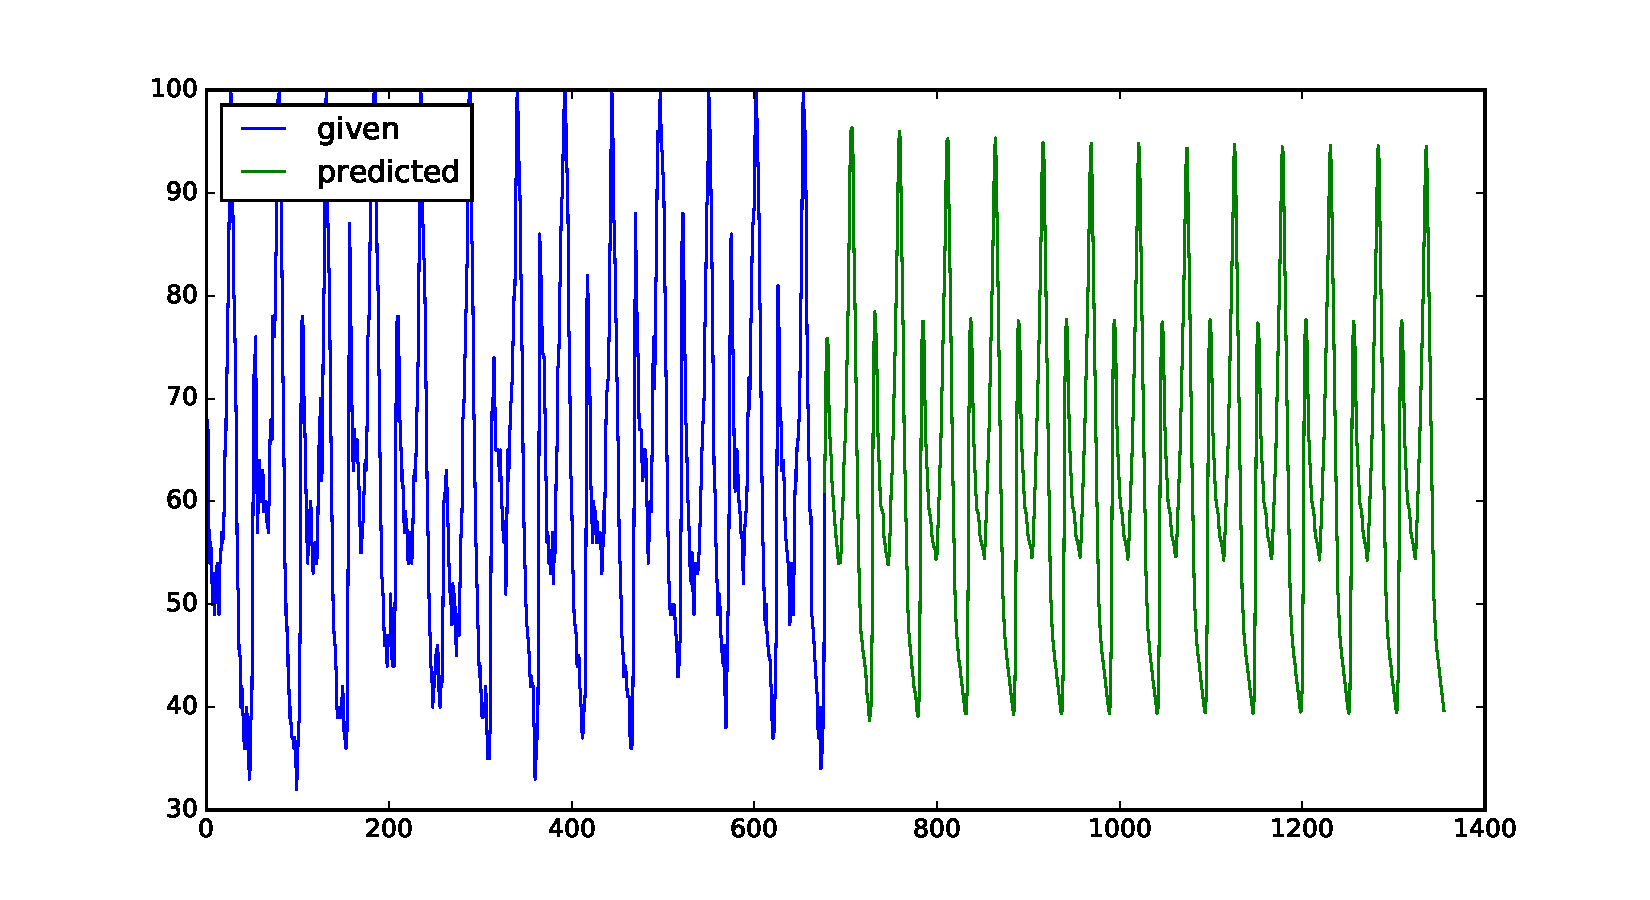
\includegraphics[width=1\textwidth]{figures/urlaub}
				\caption{google trends for term "Urlaub"}
				\label{fig:urlaub}
			\end{subfigure}	
			\caption{The prediction fit}
		\end{figure}


	
	\begin{item}
		\textbf{Recurrent Neural Network}
	\end{item}
	\begin{enumerate}
		
		%a)
		\begin{item}
			Our architecture consists of a linear layer to scale the input, followed by a lstm layer, followed by three linear layers. The number of stacked LSTMs is chosen such that it covers three consecutive sine waves to capture both the shape of the sine wave as well as the increasing amplitude. More sine waves could be covered at the cost of longer training time.
		\end{item}
		
		
		
		%b)
		\begin{item}
			A Long short-term memory (LSTM) cell utilizes a hidden state in order to calculate a prediction with each time step using information from the previous value of a given sequence.
			
		\end{item}
		
		%c)
		\begin{item}
			Training went well.
		\end{item}
		
		%d)
		\begin{item}
			The  figure \ref{fig:sine} shows the prediction fit. The network predicts the sine curve quiet smoothly, but sadly does not increase the amplitude in an expected manner. 
			To form a test dataset,  the last 100 samples were removed. 
			The mean squared error is 0.000339 and the maximum absolute difference is 0.038844 between the predicted values and the test dataset.
	
		\end{item}
		%e)
		\begin{item}
			linear -> lstm -> linear -> linear -> linear -> l2 loss
		\end{item}
		
		%f)
		\begin{item}
			The  figure \ref{fig:urlaub} shows the number of search queries for the term "Urlaub" starting in the year 2004 until now (blue) as stated by google trends, and our networks prediction (green). The trend shows strong seasonal patterns wich are predicted fairly well.
		\end{item}
	\end{enumerate}

	
\end{enumerate}

\begin{figure}[p]
	\centering
	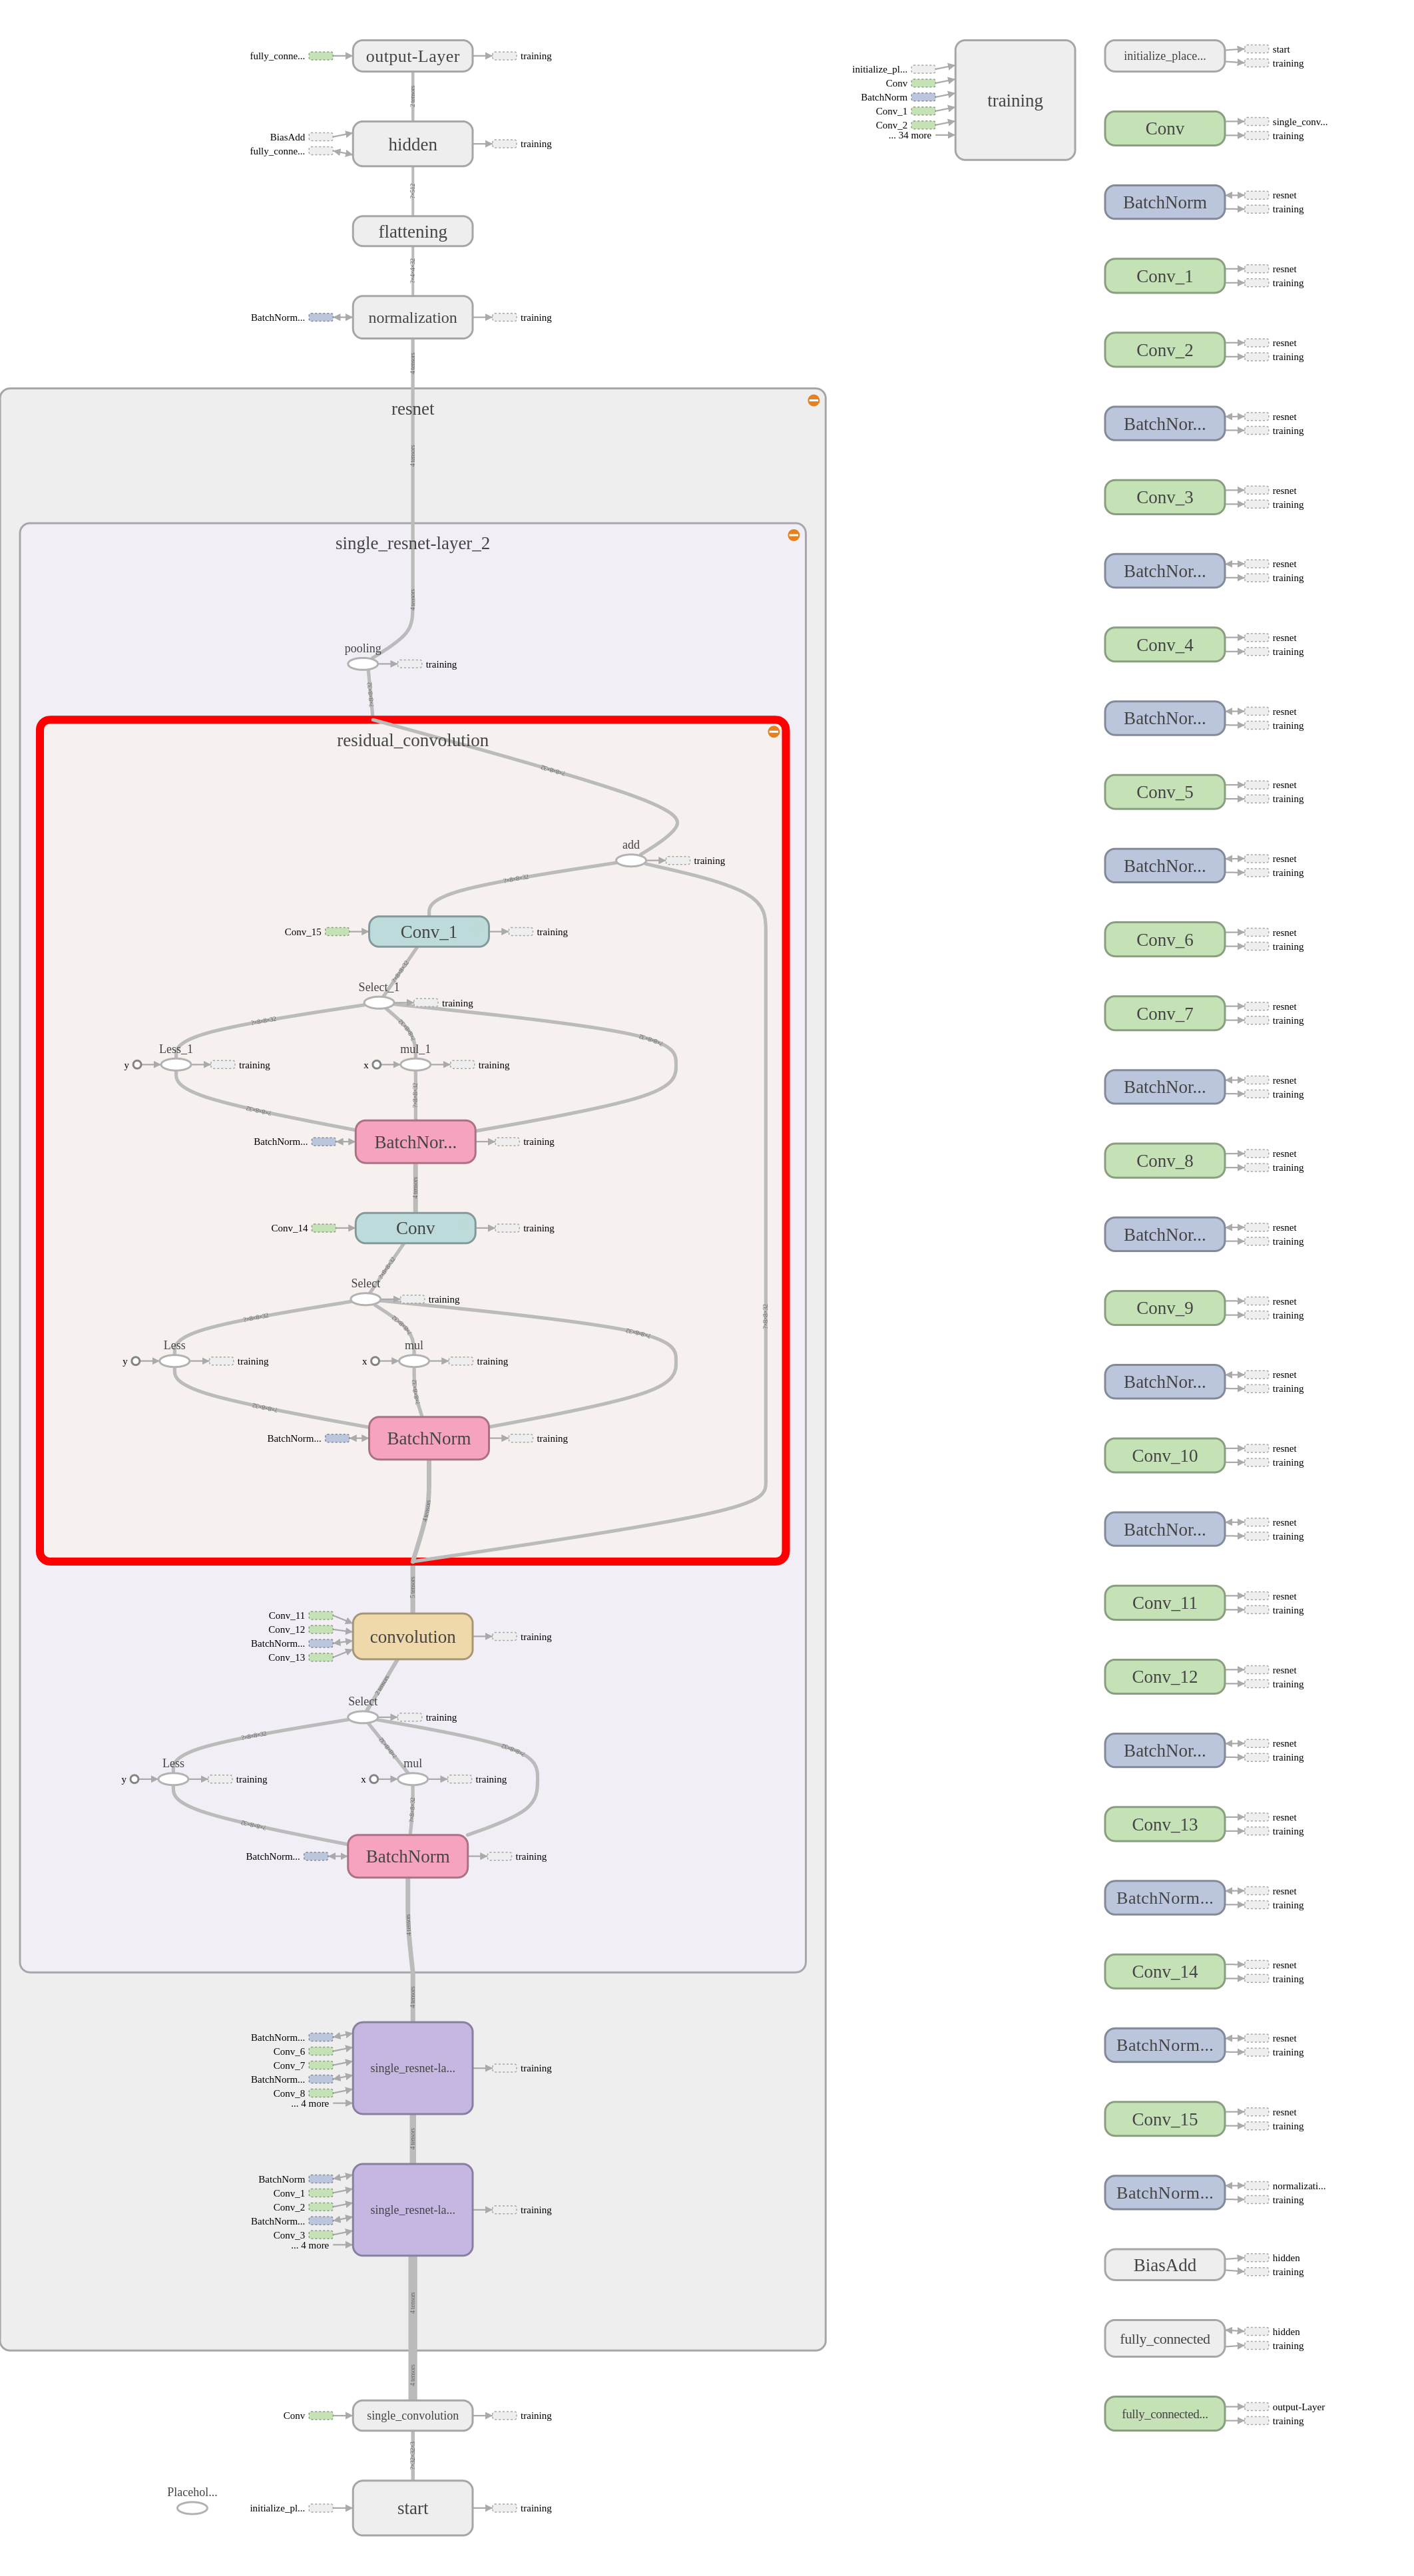
\includegraphics[width=0.6\textwidth]{figures/cifar_4_Extended}
	\caption{Tensorboard}
	\label{fig:tensorboard}
\end{figure}


\bibliography{/Users/pabrz/git/DeepLearningProjects/projects/project2/doc/citiations.bib}
\bibliographystyle{plainnat}

\end{document}
